\documentclass[../bericht.tex]{subfiles}

\begin{document}
  \chapter{Physikalische Grundlagen}


    \section{Termschema und Spektrallinien von Caesium}


      Im Versuch wird eine Gaskammer mit \ce{Cs133} verwendet. Um die erlaubten Übergänge und damit die Spektrallinien mit und ohne externes  Magnetfeld zu bestimmen müssen der normale \textsc{Zeeman} Effekt, die Feinstruktur und die Hyperfeinsturktur betrachtet werden.


      \subsection{Normaler Zeeman Effekt}
      \label{subsec:zeeman}

        Der \textsc{Zeeman} Effekt beschreibt die beobachtete Energieaufspaltung der entarteten $E_{n,l,m}$-Zustände der Elektronen in der Atomschale in $m$ Subniveaus in einem externen Magnetfeld $\vec{B}$, wobei $n,l,m$ die bekannten Quantenzahlen sind. Nach dem semiklassischen Modell bewegen sich die Elektronen auf einer Kreisbahn um den Atomkern. Hierdurch wird ein Kreisstrom und damit ein magnetisches Moment
        \begin{equation*}
          \vec{p}_m=-\frac{e}{2m_e}\cdot \vec{l},
        \end{equation*}
        mit dem Bahndrehimpuls des Elektrons $\vec{l}$, der Elementarladung $e$ und der Elektronenmasse $m_e$, erzeugt, welches mit dem Feld $\vec{B}$ wechselwirkt. Die magnetische Quantenzahl $m$ kann die Werte
        \begin{equation*}
          -l \le m \le +l
        \end{equation*}
        annehmen. Damit spalten die Energieniveaus $E_{n,l,m}$ gemä\ss
        \begin{equation}
          E_{n,l,m}=E_\mathrm{Coul}(n,l)+\underbrace{\frac{e\hslash}{2m_e}}_{=\mu_\mathrm{Bohr}}\cdot mB
        \end{equation}
        in $(2l+1)$ Komponenten auf. $\mu_\mathrm{Bohr}$ wird als \textsc{Bohr}'sches Magneton bezeichnet. Die \textit{\textsc{Zeeman}-Aufspaltung} der Spektrallinien ist unabhängig von $n,l$ und damit äquidistant
        \begin{equation}
          \Delta E=\mu_\mathrm{Bohr}\cdot B.
        \end{equation}
        Ausführlich inklusive der Erklärung der erlaubten Übergänge wird der \textsc{Zeeman} Effekt in \cite{dem:exp3-normaler-zeeman} beschrieben, obige Beschreibung enthält Auszüge.


      \subsection{Spin-Bahn-Kopplung und Feinstruktur}
      \label{subsec:feinstruktur}

        Zusätzlich zu dem aus der Bahnbewegung des Elektrons resultierenden magnetischen Moment ergibt sich aus dem quantenmechanischen Modell das magnetische Moment
        \begin{equation*}
          \vec{\mu}_s=-2\mu_\mathrm{Bohr}\frac{\vec{s}}{\hslash},
        \end{equation*}
        welchem der Spindrehimpuls $\vec{s}$ zugrunde liegt.

        Das magnetische Moment $\vec{\mu}_s$ des rotierenden Elektrons befindet sich nun im durch die Rotation erzeugten Magnetfeld $\vec{B}$. Je nach Spineinstellung führt dies zur einer Erhöhung bzw. einer Verringerung der Energie
        \begin{equation}
          \Delta E_{l,s}=-\vec{\mu}_s\cdot \vec{B}\approx \frac{\mu_0Z\cdot e^2}{8\pi m_e^4r^3}\left( \vec{s}\cdot \vec{l}\right).
          \label{eq:feinstruktur-1}
        \end{equation}
        Hierbei ist $\mu_0$ die magnetische Suszeptibilität und $Z$ die Ordnungszahl des Atoms.

        Die vektorielle Addition von Bahndrehimpuls und Spindrehimpuls ergibt den Gesamtdrehimpuls
        \begin{equation*}
          \vec{j}=\vec{l}+\vec{s}.
        \end{equation*}
        Wie Bahndrehimpuls und Spindrehimpuls ist der Gesamtdrehimpuls gequantelt. Es gilt
        \begin{equation*}
          |\vec{j}|=\sqrt{j(j+1)}\cdot \hslash
        \end{equation*}
        wobei
        \begin{equation*}
          j=+\frac{1}{2} \quad \text{für} \quad l=0
        \end{equation*}
        und
        \begin{equation*}
          j=l\pm \frac{1}{2} \quad \text{für} \quad l>0,
        \end{equation*}
        da sich die $z$-Komponenten der Drehimpulse entweder parallel oder antiparallel einstellen können.

        Nun lässt sich \eqref{eq:feinstruktur-1} umschreiben zu
        \begin{equation}
          \Delta E_{l,j}=\frac{a}{2}\cdot \left[j(j+1)-l(l+1)-s(s+1)\right]
        \end{equation}
        mit der Spin-Bahn-Kopplungskonstante
        \begin{equation*}
          a=\frac{\mu_0 Z e^2\hslash ^2}{8\pi m_e^2r^3}.
        \end{equation*}
        Die Aufspaltung der Spektrallinien gemä\ss
        \begin{equation}
          E_{n,l,j}=E_n + \Delta E_{l,j}
        \end{equation}
        ist die sogenannte \textit{Feinstrukturaufspaltung}.

        Die vorangegangenen Ausführungen sind eine Kurzfassung von \cite{dem:exp3-feinstruktur}.


      \subsection{Hyperfeinstruktur}
      \label{subsec:hyperfeinstruktur}

        Analog zum Spin des Elektrons wird auch dem räumlich ausgedehnten Atomkern ein Spin zugeordnet, der sogenannte Kernspin $\vec{I}$. Mit der Kernspinquantenzahl $I$ wird die Quantelung des Kernspins gemä\ss
        \begin{equation*}
          |\vec{I}|=\sqrt{I(I+1)}\hslash.
        \end{equation*}
        Dabei kann die Projektion auf die $z$-Richtung die $(2I+1)$ Werte
        \begin{equation*}
          I_z=m_I\cdot \hslash \quad \text{mit}\quad -I\le m_I \le +I
        \end{equation*}
        annehmen. Das magnetische Kernmoment ergibt sich damit zu
        \begin{equation*}
          \vec{\mu}_I=\gamma_\mathrm{K}\cdot \vec{I}.
        \end{equation*}
        Das magnetische Kernmoment befindet sich im vom Elektron durch Bahnbewegung und Spinmoment erzeugten Magnetfeld $B_j$ und hat hierdurch die Energie
        \begin{equation*}
          E_{I,j}=-|\mu_I|\cdot B_j \cdot \cos \left( \sphericalangle \left( \vec{j}, \vec{I}\right) \right).
        \end{equation*}
        Mit dem Gesamtdrehimpuls des Atoms
        \begin{equation*}
          \vec{F} = \vec{j}+\vec{I}
        \end{equation*}
        spaltet sich damit jedes Energieniveau der Feinstruktur in der \textit{Hyperfeinstruktur} nach
        \begin{equation}
          E_{HFS}=E{n,l,j} + \frac{A}{2}\left[ F(F+1) - j(j+1) - I(I+1) \right],
        \end{equation}
        mit der Hyperfeinkonstante
        \begin{equation*}
          A=\frac{g_I \cdot \mu_\mathrm{K}\cdot B_j}{\sqrt{j(j+1)}},
        \end{equation*}
        auf. Die vollständige Herleitung ist in \cite{dem:exp3-hyperfeinstruktur} zu finden.


      \subsection{Termschema von Cäsium}
      \label{subsec:termschema-caesium}

        Die Elektronen der Atome können von ihrem Grundzustand in energiereichere Zustände angeregt werden. Da alle Zustände diskret sind ergibt sich ein Termschema wie in \cref{fig:termschema}. Allerdings gibt es Auswahlregeln für die möglichen Übergänge. Für Übergänge muss gelten: $\Delta m= \pm 1$ oder 0 und $\Delta l=\pm 1$. Ausführlichere Ausführungen sind in \cite{grif:quanten} zu finden.

        Für dieses Experiment interessiert die Anregung des Grundzustands $6^2\mathrm{S}_{1/2}$ in den $6^2\mathrm{P}_{3/2}$-Zustand.
        \begin{figure}[tb]
          \begin{center}
            \fbox
            {
            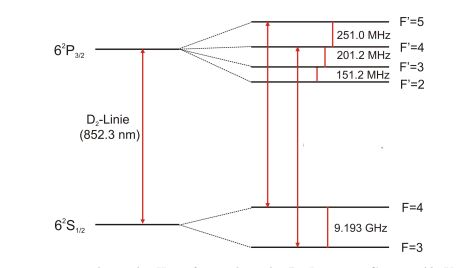
\includegraphics[angle=0, height=8 cm]{figures/fein-hyp.JPG}
            }
            \caption{Teil des Termschemata von Cäsium, mit Fein- und Hyperfeinstruktur (\cite{fein-hyp}). }
          \end{center}
          \label{fig:termschema}
        \end{figure}




    \section{Spektrallinienverbreiterung}
    \label{sec:linienverbreiterung}

      Die im vorherigen Abschnitt bestimmten Spektrallinien werden experimentell nur in verbreiterter Form gemessen. Dieser Linienverbreiterung liegen die natürliche Linienbreite, die Dopplerverbreiterung und die Druckverbreiterung zu Grunde.

      \subsection{Natürliche Linienbreite}
      \label{subsec:natuerliche-linienbreite}

        Aufgrund der Unschärferelation kann kein physikalischen System gleichzeitig eine scharf definierte Energie und sich verändern. Da ein Übergang eine Veränderung darstellt kann dessen Energie also nicht scharf definiert sein. Somit liegt eine Linienverbreiterung vor.


      \subsection{Dopplerverbreiterung}
      \label{subsec:dopplerverbreiterung}

        Da sich die Atome in der Gaskammer bewegen kommt es in Abhängigkeit von der Bewegung parallel zur Strahlrichtung nach dem \textsc{Doppler} Effekt zu einer Rot-, bzw. einer Blauverschiebung. Diese Linienverbreiterung wird Dopplerverbreiterung genannt.


      \subsection{Druckverbreiterung}
      \label{subsec:druckverbreiterung}

        Je nach Gasdruck in der Gaskammer kommt es zu mehr oder weniger Stö{\ss}en zwischen den Cäsium-Atomen. Die Wechselwirkung zwischen den Atomen beeinflusst das Termschema und verbreitert damit die Linien. Die Linienverbreiterung ist proportional zum Druck, weshalb idealerweise der Gasdruck in der Gaskammer sehr niedrig ist.


    \section{Dopplerfreie Spektroskopie}

      Für die \textsc{Doppler}freie Spektroskopie werden zwei antiparallele Laserstrahlen genutzt. Diese können, wie in diesem Experiment, vom selben Laser stammen. Ein Strahl, der \textit{Pumpstrahl}, zeichnet sich durch seine höhere Intensität im Vergleich zum zweiten Strahl aus. Letzterer wird als \textit{Abfragestrahl} bezeichnet.
      Im Falle einer Strahlteilung eines einzelnen Lasers haben beide Strahlen die gleiche Wellenlänge $\lambda_0$, bzw. Frequenz $f_0$. Im Bezugssystem eines Atoms mit Geschwindigkeitskomponente parallel zum Strahlengang $v_z$ haben die beiden antiparallelen Laserstrahlen unterschiedliche Wellenlängen $\lambda ^{-,+}$ gemä\ss
      \begin{equation*}
        v_z^-=\lambda^- (f-f_0),\quad v_z^+=-\lambda^+ (f-f_0).
      \end{equation*}
      \medskip
      Wenn die Frequenz des Laserstrahls im Laborsystem von der Resonanzfrequenz $f_\mathrm{r}$ der Atome abweicht, d.h. $f_0\ne f_\mathrm{r}$, dann werden alle Teilchen der Geschwindigkeit $|v_z^\mathrm{r}|$ angeregt. Aufgrund der entgegengesetzten Bewegungsrichtung sind beim Pump- und beim Sättigungsstrahl jeweils ein Minimum an Stelle des unteren Energieniveaus im dopplerverbreiterten Profil und ein Maximum an Stelle des oberen (angeregten) Ernergieniveaus. Die Minima werden \textsc{Bennet}-Löcher genannt.
      \medskip

      Im Fall $f_0 = f_\mathrm{r}$ absorbieren die Atome mit Geschwindigkeitskomponente $v_z^\mathrm{r} = 0$. Hierbei überlagern sich die beiden \textsc{Bennet}-Löcher. Nun wird das Profil des \textit{Abfragestrahls} zwei mal gemessen: Einmal ohne \textit{Pumpstrahl} und einmal mit. Ohne erscheint das dopplerverbreiterte Profil. Bei eingeschaltetem \textit{Pumpstrahl} wird durch dessen hohe Intensität das untere Energieniveau entvölkert und das obere gesättigt. Als Folge dessen weist das Profil des \textit{Abfragestrahls} nun Minima an Stelle der Absorptionslinien auf, sogenannte \textit{\textsc{Lamb}-Dips}. Durch Differenzbildung der beiden Profile entsteht so ein dopplerfreies Absorptionsspektrum der Atome.

      Dieser Aufbau zur dopplerfreien Spektroskopie wird auch \textit{Sättigungsspektroskopie} genannt.


    \section{Cross-over Resonanz}

      Wenn zwei Absorptionskurven so nahe aneinander liegen, dass sich die Dopplerprofile überlagern tritt die sogenannte Cross-over Resonanz auf. Wenn für Pumpfrequenz $\nu$ und die Resonanzfrequenzen $\nu_1$, $\nu_2$ gilt,
      \begin{align*}
        \nu_2 - \nu = \nu - \nu_1 = \pm \frac{v^*}{c} \nu_0
      \end{align*}
      wechselwirken die Laserstrahlen mit Atomen mit der Geschwindigkeit $v^*$. Dadurch entsteht ein drittes Minimum im Absorptionsspektrum zwischen den beiden anderen.

    \section{Diodenlaser}

      Es folgt eine Kurzfassung von \cite{quant} zur Funktion von Diodenlasern.

      Diodenlaser sind aus Halbleitern aufgebaut. Der Laserlicht entsteht wenn sich die Elektronen im Leitungsband mit den Löchern im Valenzband rekombinieren.
      \begin{figure}[tb]
        \begin{center}
          \fbox
          {
          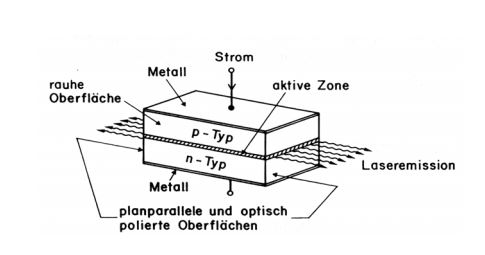
\includegraphics[angle=0, height=6 cm]{figures/diodenlaser.JPG}
          }
          \caption{Schematischer Aufbau eines typischen Diodenlasers (\cite{quant}). }
          \label{fig:diodenlaser}
        \end{center}
      \end{figure}

      Wie in \cref{fig:diodenlaser} zu sehen ist, besteht der Hauptteil eines Diodenlasers aus einem $p-n$-Übergang, der durch Dotierung erzeugt wird. Das anlegen einer Spannung führt zu einer Besetzungsinversion mit Löchern im Valenzband und Elektronen im Leitungsband. Dies ist der Pumpprozess des Lasers. Die Rekombination der Löcher und Elektronen kann spontan oder stimuliert erfolgen. Das dabei emittierte Licht ist nur Kohärent falls die stimulierte Emission überwiegt.
      Aufgrund des hohen Brechungsindexes der Halbleiterkristalle fungieren sie direkt als Resonatoren. Die Seite auf der kein Licht austreten soll wird verspiegelt. Die Endfläche des Kristalls hatte eine Reflektivität von ca. $\SI{30}{\percent}$. Aufgrund der hohen Verstärkung reicht dies aus. Wie für Resonatoren üblich gilt für die sich ausbildenden stehenden Wellen:
      \begin{align*}
        L=m\cdot\frac{\lambda}{2n}
      \end{align*}
      Hierbei ist $m$ eine natürliche Zahl, $n$ der Brechungsindex, $\lambda$ die Wellenlänge und $L$ die Länge des Resonators/ Kristalls.\\
      Vorteile dieses Lasers sind das einfache Pumpen, seine relativ starke Leistung sowie die Durchstimmbarkeit der Frequenzen in gewissen Grenzen. Außerdem ist er klein, billig und hält langen Gebrauch gut aus.


    \section{Konfokales Fabry-Perot-Etalon}

      Ein konfokales \textsc{Fabry-Perot}-Etalon ist ein Interferometer aufgebaut aus zwei sphärischen Spiegeln. Die sphärischen Spiegel reduzieren die Empfindlichkeit des Strahls auf Justierungen am Spiegel und reduzieren Beugungsverluste. Aufbau und Strahlenverlauf sind in \cref{fig:fabry-perot} zu sehen.
      \begin{figure}
        \begin{center}
        \fbox
        {
          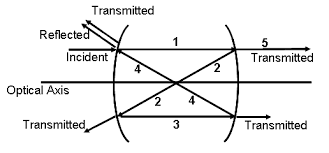
\includegraphics[angle=0, height=6 cm]{figures/fabryperot}
        }
        \caption{Strahlengang in einem konfokalen \textsc{Fabry-Perot}-Etalon (\cite{fabry-perot}).}
        \label{fig:fabry-perot}
        \end{center}
      \end{figure}
      Nach vier Reflektionen kommt der Strahl wieder am Ausgangspunkt an. Wenn die Strahlen 0, 4, 8, 12, ... mal reflektiert wurden und dann an der gleichen Stelle transmittieren kommt es zu Interferenz. Der Krümmungsradius und der Abstand zwischen den Spiegeln ist r. Wenn für die Abstände zwischen den Reflektionspunkten und der optischen Achse gilt $\rho_1$ und $\rho_2 \ll r$ und der Eintrittswinkel gilt $\theta \ll 1$, dann ist die Bedingung für konstruktive Interferenz durch
      \begin{align*}
        4r+\frac{\rho_1^2\cdot\rho_2^2}{r^3}\approx4r=m\lambda.
      \end{align*}
      gegeben.

      Obige Beschreibungen sind an die detaillierteren Ausführungen in \cite{dem:laser} angelehnt.








\end{document}
